\chapter{Architektury přístupových systémů}
Přístupové systémy jsou elektronické systémy řídící přístup uživatelů do omezených prostor v závislosti na jejich prokázané identitě.
 
\begin{figure}[!h]
    \centering
    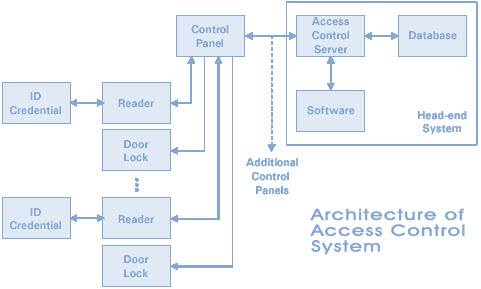
\includegraphics[width=80mm]{Architetcture-of-Access-Control-System}
    \caption{Příklad architektury přístupového systému \cite{accessControlSystem_eiprocus}}
    \label{fig:Access control system architecture}
\end{figure}

Obrázek \ref{fig:Access control system architecture} zobrazuje typickou architekturu přístupového systému, kde ID Credential představuje prvek ůmožňující identifikovat uživatele, např. RFID tag, otisk prstu nebo QR kód. 
Reader slouží ke čtení dat z ID Credential a v digitální podobě je pošle k zařízení typu Control Panel.
Zařízení Door Lock řídí fyzický přístup uživatelů do omezených prostor. 
Zařízení typu Control Panel tvoří rozhranní mezi Access Control Server a páry zařízení typů Reader a Door Lock. 
Zařízení typu Control Panel jsou obvykle připojena 
k zařízení typu Access Control Server přes TCP/IP síť.
A páry zařízení Reader a Door Lock jsou obvykle připojeny k zařízení typu Control panel přes RS485 síť, jehož hlavním účelem je řízení těchto párů. Databáze obsahuje všechny uživatelské ID.
Na Access Control Serveru je spuštěn Software (SW) spravující databázi a komunikující se všemi zařízeními typu Contril Panel.
Zařízení typu Reader čte uživatelská ID z předložených ID Credential uživateli a přeposílá je k zařízení typu Control Panel, které je dále přeposílá na Access Control Server. Access Control Software vyhledá obdržená uživatelská ID v databáze a pokud je nalezeno, pošle příkaz odpovídajícímu zařízení typu Control Panel k přepnutí odpovídajícímu zařízení typu Door Lock \cite{accessControlSystem_eiprocus}.
